\begin{figure}[!ht]
	\centering
	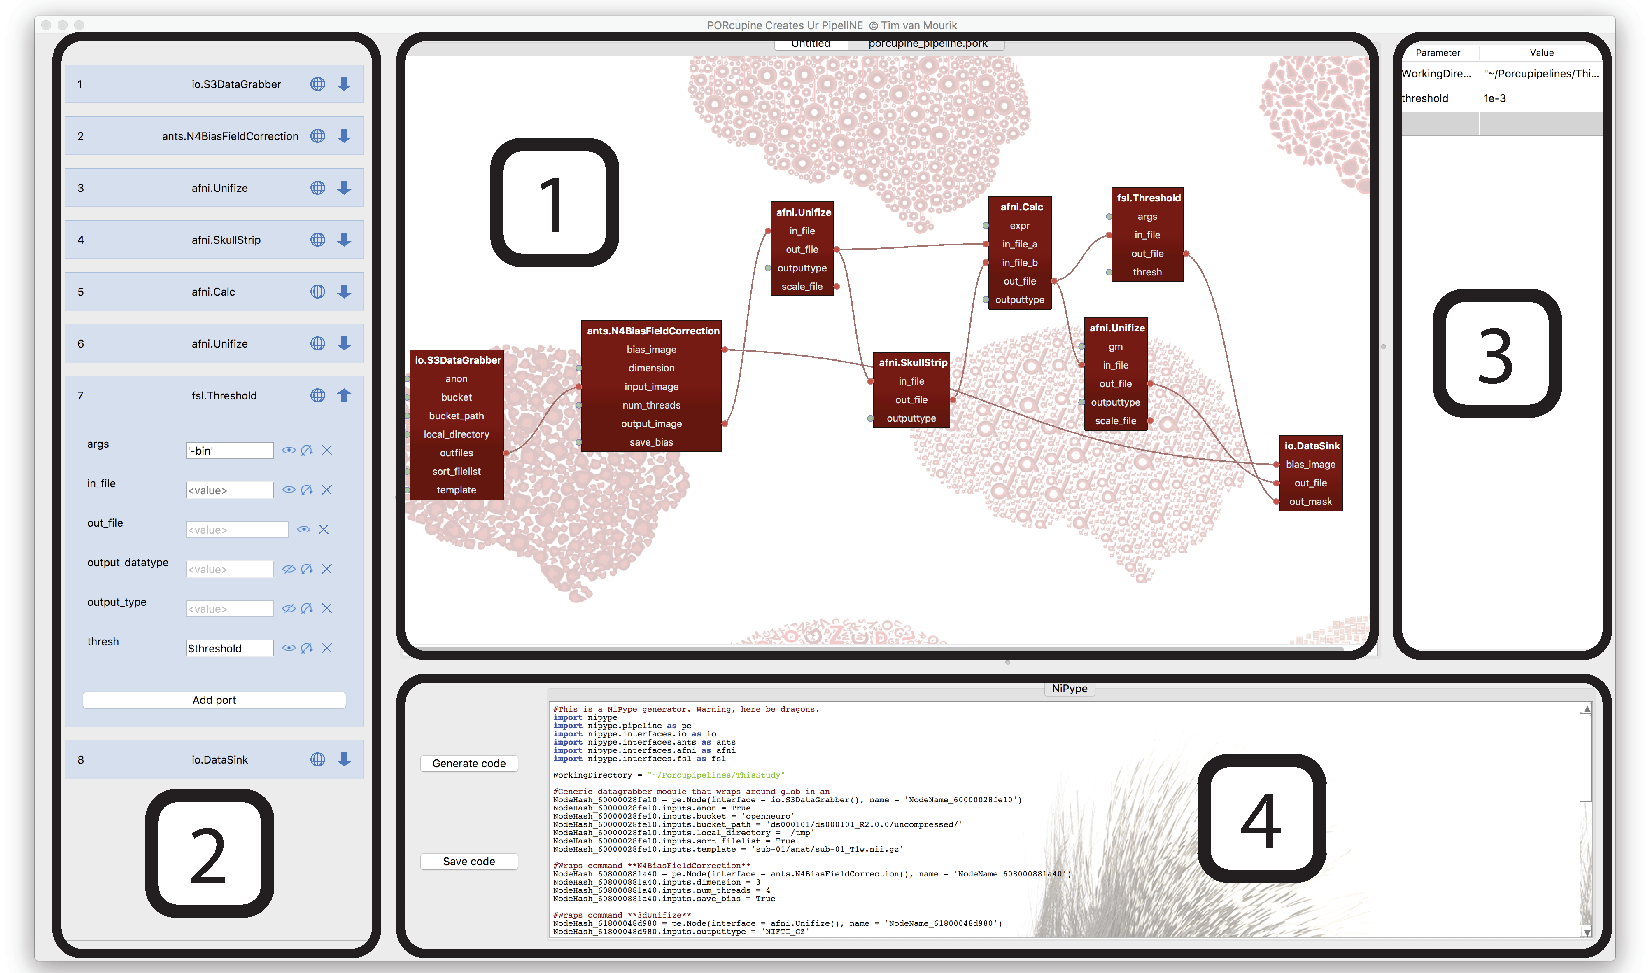
\includegraphics[width=0.9\textwidth, clip=true]{./Chapters/05_Porcupine/./Images/gui_showcase.pdf}
	\caption{A screenshot of a Porcupine workflow. The editor is divided into four panels, each of them targeted at facilitating a more understandable and reproducible analysis. The \emph{workflow editor} (1) provides a visual overview of one's analysis. The functions are all listed in the \emph{node editor} (2), where the parameters for all functions can be orderly stored. This may include links to important parameters that are listed in the \emph{parameter editor} (3), such that an overview of the main analysis settings can be easily viewed and modified. Readily executable analysis code is generated in the \emph{code window} (4)}
	\label{fig:porcupine-editor}
\end{figure}